\chapter{Design and Implementation}
\label{ch:design_implementation}
This chapter describes the design and implementation of the delegation mechanisms integrated into vodle, detailing both the technical approach and practical decisions made throughout development. It begins by outlining vodle's existing system architecture, clarifying how this influenced the integration of new delegation features. 

Each subsequent section aligns directly with one of the project objectives defined previously, explaining the rationale behind key design choices, algorithms, and interface elements. Emphasis is placed on the critical design trade-offs and challenges encountered, highlighting how constraints such as the serverless architecture and client-side computation informed implementation decisions.

\section{System Architecture Overview}\label{sec:design_architecture}
Vodle is built as a serverless web application that emphasises accessibility, client-side performance, and ease of deployment. Its architecture comprises two components:

\begin{enumerate}
  \item \textbf{Frontend:} Implemented using Angular and the Ionic framework, the frontend provides a responsive and modular interface that works across both desktop and mobile devices. The use of Angular facilitates the creation of component-based user interfaces, essential for introducing interactive features such as the ranked delegation UI and weighted delegation sliders.
  \item \textbf{Backend:} Vodle uses CouchDB as its database. There is no custom backend logic or middleware
  %\footnote{Except for a small number of permission management scripts implemented directly in CouchDB via CouchDB ``design functions''.};
  instead, the frontend application communicates directly with CouchDB over HTTP.
\end{enumerate}

\subsubsection{Implications of This Architecture}
Vodle's serverless architecture has several implications for the design and implementation of the delegation mechanisms, especially due to the absence of a traditional data processing backend. The following points summarise the key considerations:
\begin{itemize}
  \item All vote delegation logic, including transitive resolution, cycle detection, and weighted delegation calculations, must be executed in the browser. This places constraints on performance and requires careful optimisation of algorithms used.
  \item CouchDB's document-based storage model means that all data must be serialised and deserialised in JSON format. This affects how data structures are designed and manipulated, as well as how they are stored and retrieved from the database.
\end{itemize}

\subsubsection{Write Validation and Constraints}
CouchDB enforces document-level security: users may only modify their own documents, and core artefacts (such as \texttt{poll.json} and results) are immutable once created. All updates must replace the full document in a single operation, with no support for merging concurrent changes.

This model simplifies validation logic, but it also imposes important constraints on implementing liquid democracy features. In particular, updating delegations or splitting votes requires replacing a user's entire vote document in a single, atomic write. This means that incremental updates (e.g., adjusting part of a delegation tree or partially reassigning vote weights) are not possible; the client must construct and submit a complete new version of the user's voting data each time. These constraints influenced both the design of weighted-delegation algorithms and the structure of delegation management within vodle.

\subsection{Summary of Storage and Validation Constraints}
\label{subsec:summary_storage_constraints}

The architecture of vodle, particularly its reliance on CouchDB and the absence of a custom backend, imposes important constraints on how delegation features are designed and implemented.

\begin{itemize}
  \item \textbf{User autonomy is strictly enforced.} Each user can only modify documents that are explicitly associated with their own identity. This guarantees that vote and delegation data cannot be tampered with by other clients but also eliminates the possibility of directly setting or managing another user's vote.

  \item \textbf{Issues with sharing a document.} The current database design does not support the modification of a single document by multiple users. As a result, features that require a global view -- such as a delegation graph -- require a rework of the database schema.

  \item \textbf{Validation logic is structural, not contextual.} Since CouchDB validation functions can only inspect the document being written, they cannot reason about relationships across documents. This prohibits logic such as resolving delegations server-side, enforcing uniqueness of votes, or validating delegation cycles at the point of write.

  \item \textbf{Client-side logic carries the burden.} Due to the previous point, all logic for delegation resolution, cycle checking, and weighted delegation must be implemented in the client. This requires careful design to ensure that the frontend can handle complex delegation scenarios without overwhelming the user or causing performance issues.
\end{itemize}

Together, these constraints shape some of the design and implementation choices of the delegation features in vodle, which will be discussed in detail in the following sections.

\section{Implement a Core Delegation Model into vodle}\label{sec:core_delegation_detailed}
This section outlines the design and implementation of the core delegation model within vodle, addressing Objective 1 of the project. It begins with an analysis of the pre-existing, partially implemented delegation system, identifying the limitations that motivated a full redesign. The second half of the section describes the final implementation, including the new data structures, algorithms, and interface improvements introduced.

\subsection{Limitations of the Pre-existing Implementation}

Before this project began, vodle included a partially implemented delegation system. Although disabled due to critical flaws, the system introduced several foundational ideas and structures that influenced the final design. This section introduces the key data structures used in the original model, explains the intended delegation flow, and analyses why a redesign was necessary.

\subsubsection*{Delegation Maps}

The delegation mechanism relied on several maps to track how votes were delegated and resolved. These maps were stored and updated locally on each client:

\begin{itemize}
    \item \textbf{direct\_delegation\_map}: This map recorded direct delegation relationships. For each option ID (\texttt{oid}), it stored a mapping from voter IDs to the user they directly delegated to.

    \item \textbf{effective\_delegation\_map}: This map stored the final casting voter for each user by resolving the full transitive chain of delegations. For example, if user A delegated to B and B delegated to C, the effective delegate of A was C.

    \item \textbf{inv\_effective\_delegation\_map}: The inverse of the effective map. For each user, it stored the set of voters whose votes were ultimately counted under them. This was useful for computing voting weights and for cycle detection.
\end{itemize}

Each map was maintained locally by the browser and not synchronised across clients. This made the correctness of delegation state dependent on each user's local view.

\subsubsection*{Delegation Flow}

Delegation in vodle followed an explicit, link-based invitation model:

\begin{enumerate}
    \item A user (the delegator) generated a delegation ID (DID), created a key pair, and constructed a \texttt{del\_request} object specifying the options to delegate.
    \item A magic link containing this information was shared with the intended delegate.
    \item The delegate could accept or reject the invitation. If accepted, a signed \texttt{del\_response} was created, completing the delegation handshake.
    \item Once accepted, a \texttt{del\_agreement} object was created and cached by both parties. This structure tracked which options were accepted and which were currently active.
\end{enumerate}

This invitation model upheld user autonomy: users could not be delegated to without their explicit consent. Delegation could also be revoked at any time and overridden on a per-option basis.

\begin{figure}[H]
  \centering
  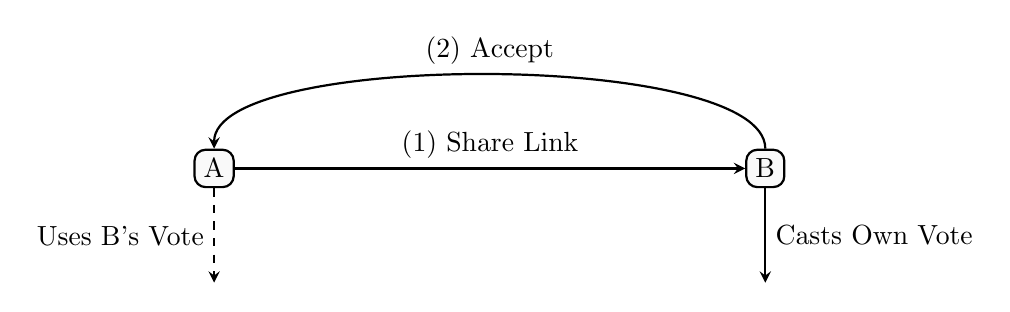
\begin{tikzpicture}[node distance=7cm,>=stealth,thick]
    % clients
    \node[rectangle,draw,rounded corners,fill=gray!5] (A) {A};
    \node[rectangle,draw,rounded corners,fill=gray!5,right of=A] (B) {B};
    % arrows
    \draw[->] (A) -- node[above]{(1) Share Link} (B);
    \draw[->] (B) .. controls +(0,1.5) and +(0,1.5) .. node[above]{(2) Accept} (A);
    \draw[->] (B.south) -- ++(0,-1.2) node[midway,right]{Casts Own Vote};
    \draw[->, dashed] (A.south) -- ++(0,-1.2) node[midway,left]{Uses B's Vote};
  \end{tikzpicture}
  \caption{Sequence for a delegation to be initiated. User A shares a link with user B, who accepts the delegation.}
  \label{fig:delegation-flow-accept}
\end{figure}

\begin{figure}[H]
  \centering
  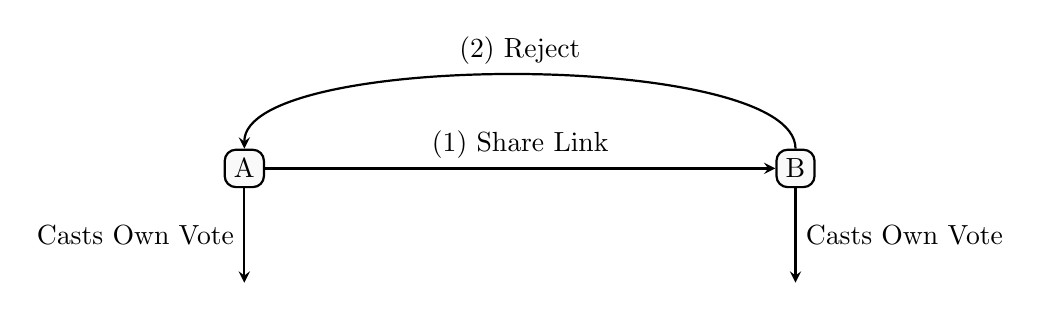
\begin{tikzpicture}[node distance=7cm,>=stealth,thick]
    % clients
    \node[rectangle,draw,rounded corners,fill=gray!5] (A) {A};
    \node[rectangle,draw,rounded corners,fill=gray!5,right of=A] (B) {B};
    % arrows
    \draw[->] (A) -- node[above]{(1) Share Link} (B);
    \draw[->] (B) .. controls +(0,1.5) and +(0,1.5) .. node[above]{(2) Reject} (A);
    \draw[->] (B.south) -- ++(0,-1.2) node[midway,right]{Casts Own Vote};
    \draw[->] (A.south) -- ++(0,-1.2) node[midway,left]{Casts Own Vote};
  \end{tikzpicture}
  \caption{Sequence for a rejected delegation. User A shares a delegation link with user B, who rejects the delegation.}
  \label{fig:delegation-flow-reject}
\end{figure}


\subsubsection*{Cycle Detection Failures}

The main flaw in the system was its inability to reliably prevent delegation cycles. A cycle occurs when a user indirectly delegates back to themselves, such as in the sequence A~$\rightarrow$~B~$\rightarrow$~C~$\rightarrow$~A. In such cases, the vote becomes trapped and is not cast.

Clients attempted to detect cycles during the delegation acceptance phase by examining local delegation maps. A typical check would confirm whether the proposed delegate was already an effective delegate of the user. If so, the client marked the request as cyclic and blocked it.

However, because these maps were not synchronised, different clients could hold conflicting views of the delegation graph. A delegation that passed validation on one device might cause a cycle once accepted, or be silently invalidated by another. This undermined correctness and made vote resolution unpredictable.

\subsubsection*{User Interface Limitations -- TODO}

\subsubsection*{Summary}

The original delegation system implemented many strong conceptual ideas. It preserved user autonomy through an invitation model, allowed for control over which options used the delegated rating, and supported transitive delegation. However, it relied entirely on client-local data and logic. Without a global, synchronised delegation graph, the system could not reliably detect cycles or ensure consistent resolution of votes. These limitations made it unsuitable for deployment and motivated a full redesign, described in the next section.

\subsection{Revised Implementation}
This section describes the final design and implementation of the core delegation mechanism in vodle, which allows users to delegate their votes to others. It addresses the limitations of the original system by introducing a global, synchronised delegation graph, efficient cycle prevention, and consistent transitive resolution logic. The design preserves the invitation-based flow and per-option control from the earlier implementation while ensuring correctness across all clients.

\subsubsection*{Cycle Checking: Algorithm and Rationale}
We can represent delegation relationships as a directed graph, where users are nodes and delegations form directed edges. A valid vote delegation must not introduce cycles in this graph: for example, a sequence such as A~$\rightarrow$~B~$\rightarrow$~C~$\rightarrow$~A would result in all votes becoming trapped, with no final casting voter. Therefore, delegation cycles must be proactively prevented at the time a new delegation is proposed.

A proposed delegation from user $X$ to user $Y$ is valid if and only if $Y$ is not a descendant of $X$ in the current delegation graph. That is, there must be no existing path from $Y$ back to $X$.

% \subsection*{Delegation Graph and Cycle Checking}\label{subsec:obj1_cycle_checking}
% Delegations are represented as a directed graph, where each user is a node and each delegation is a directed edge from a delegator to their delegate. Preventing cycles in this graph is essential to guarantee that every vote can be correctly resolved to a casting user.

% Rather than recomputing the full graph for each delegation attempt, the algorithm maintains a data structure called the \texttt{inverse\_indirect\_map}, which stores the transitive descendants of each user.

Instead of checking for this condition directly using a depth-first search (DFS) or breadth-first search (BFS), a more efficient approach is to maintain a list of all descendants for each user. This allows us to check if $Y$ is in the list of descendants of $X$ in constant time. The implementation details of this approach is detailed in the next section.

\subsubsection{Implementation Details}
A hashmap is used to store the descendants of each user. The keys are user IDs, and the values are sets of user IDs representing the direct delegates of that user. In the code, this hashmap is referred to as ``\verb|inverse_indirect_map|''.

Suppose the following delegations exist:
\begin{itemize}
    \item A delegates to B
    \item B delegates to C
    \item C delegates to D
\end{itemize}

The resulting \texttt{inverse\_indirect\_map} is:
\begin{figure}[H]
  \centering
  \begin{minted}{python}
    inverse_indirect_map = {
      "B": {"A"},
      "C": {"B", "A"},
      "D": {"C", "B", "A"}
    }
    \end{minted}
  %\caption{Example of a hashmap for users A, B, C, and D. User A has delegated to B, user B has delegated to C, and user C has delegated to D. Consequently, the descendants of user D are A, B and C.}
  \label{fig:inverse_indirect_map}
\end{figure}

This map enables several key operations required for maintaining a consistent and cycle-free delegation graph:

\begin{itemize}
  \item \textbf{Check Delegation Validity:} To determine whether a delegation \(X \!\to\! Y\) would create a cycle, the system checks if \(Y\) already appears in the set of descendants of \(X\). If so, the new delegation is invalid. This check takes \(O(1)\) time.
  \begin{figure}[H]
    \centering
    \begin{minted}{javascript}
      const inverse_indirect_map = this.G.D.get_inverse_indirect_map(pid);
      const descendant_set = inverse_indirect_map.get(delegate_vid);
      if (descendant_set.has(myvid)) {
        cycle = true;
      }
    \end{minted}
    \caption{Code for checking if a delegation is valid. This check is triggered when a user clicks on a delegate link. The map is retrieved from the synchronised local cache, and the set of descendants is used to confirm that a cycle would not be formed.}
  \end{figure}

  \item \textbf{Add Delegation Edge:} When a new delegation \(X \to Y\) is accepted, the system must ensure that the descendant relationship is updated consistently. Specifically, for $Y$ and every user \(u\) such that \(Y \in \texttt{desc}(u)\), their descendants must be updated to include both \(X\) and all of \(X\)'s current descendants.

  \item \textbf{Remove Delegation Edge:} When a delegation \(X \!\to\! Y\) is removed, the system must ensure that the descendant relationship is updated consistently. Specifically, for $Y$ and every user \(u\) such that \(Y \in \texttt{desc}(u)\), their descendants must be updated to remove both \(X\) and all of \(X\)'s current descendants.
\end{itemize}

\subsubsection{User Interface -- TODO: add screenshots and actually fill in}
\begin{itemize}
\item Create delegation invite line
\item Accept screen
\item Accept screen when there is a cycle
\item UI from user A POV (votes are being controlled)
\begin{itemize}
  \item Note Fixes:
  \item controls some-all-none of your votes
  \item your vote is used for n-other delegates
\end{itemize}
\item UI from user B POV (Is a delegate)
\end{itemize}

\begin{figure}[H]
  \centering
  \begin{subfigure}[t]{0.28\linewidth}
    \centering
    \includegraphics[width=\linewidth]{../common/initial_vodle_screenshots/deldialog.png}
    \caption{User A's invitation screen.}
    \label{fig:del-dialog}
  \end{subfigure}
  \hfill
  \begin{subfigure}[b]{0.68\linewidth}
    \centering
    \includegraphics[width=\linewidth]{../common/initial_vodle_screenshots/delaccept.png}
    \caption{User B's delegation acceptance screen when there is no cycle.}
    \label{fig:del-accept}
    
    \vspace{1em}
    
    \includegraphics[width=\linewidth]{../common/initial_vodle_screenshots/delaccept_cycle.png}
    \caption{User A's screen after opening a delegation link from User C (who User B has delegated to).}
    \label{fig:del-accept-cycle}
  \end{subfigure}
  \caption{Screens shown to Users A and B during the delegation invitation and response process.}
  \label{fig:delegation-accept-flow}
\end{figure}


\begin{figure}[H]
  \centering
  \begin{subfigure}[t]{0.8\linewidth}
    \centering
    \includegraphics[width=\linewidth]{../common/vodle_screenshots/userA_after.png}
    \caption{User A (delegator) can now see that their waps are controlled by User B.}
    \label{fig:userA_after}
  \end{subfigure}

  \vspace{1em}

  \begin{subfigure}[t]{0.8\linewidth}
    \centering
    \includegraphics[width=\linewidth]{../common/initial_vodle_screenshots/userB_after.png}
    \caption{User B (delegate) can see that their vote also determines the outcome for one other user (User A).}
    \label{fig:userB_after}
  \end{subfigure}

  \caption{Delegate's (bottom) and delegator's (top) screens after a delegation has been accepted.}
  \label{fig:delegation_flow_ui}
\end{figure}
\subsection{Summary -- TODO}

\section{Implement Ranked Delegation into Vodle}\label{sec:design_ranked_delegation}

This section describes the design and implementation of ranked delegation in vodle, addressing Objective 2 of the project. The ranked delegation system allows users to specify fallback delegates in case their primary delegate is unavailable due to abstaining or being part of a cycle.

The implementation of ranked delegation in vodle is poll-specific: each user may specify a ranked list of up to three delegates for a given poll. These preferences are evaluated using the MinSum delegation rule (see Section~\ref{subsec:background_ranked_delegation}), which selects the delegation path with the lowest cumulative rank cost. This ensures that the system respects the user's stated preferences as closely as possible, while avoiding unnecessarily long or indirect delegation chains.

\subsection{Data Structures}
Each voter's ranked delegates are stored in the \texttt{direct\_delegation\_map}, which maps a user ID to a list of delegation entries. Each entry is a triple:
\[
[\text{delegate\_id}, \text{rank}, \text{status}]
\]
where:
\begin{itemize}
    \item \texttt{delegate\_id} is the user ID of the delegate.
    \item \texttt{rank} is the position in the ranking (1 = most preferred).
    \item \texttt{status} indicates whether the delegation is accepted (1), pending (0), rejected (0), or active (2).
\end{itemize}

This new map was necessary because the existing \texttt{inverse_indirect_map}, used for cycle detection, only tracked resolved descendant relationships and did not retain information about alternative delegation paths or their ranks. Ranked delegation, by contrast, required maintaining multiple potential delegates per user, their relative preferences, and their acceptance statuses. Without a dedicated structure like \texttt{direct_delegation_map}, it would not have been possible to correctly resolve delegation paths according to user preferences using the MinSum rule.

For example, if only User A has delegated and they rank User B first, User C second, and User D third, and B and C accept the delegation while D does not respond, the resulting structure is:

\begin{figure}[H]
  \begin{minted}{python}
    direct_delegation_map = {
      "A": [["B", 1, 2], ["C", 2, 1], ["D", 3, 0]]
    }
  \end{minted}
  \caption{Example of a \texttt{direct\_delegation\_map} entry for ranked delegation. B is marked as active as the path $A\to B$ has the lowest total sum of ranks.}
\end{figure}

\subsection{Delegation Resolution Using MinSum}

Whenever a delegation is accepted, rejected, or revoked, all paths must be recomputed using the MinSum rule. This ensures that the voting power of each user flows through the most appropriate path.

The MinSum algorithm is implemented as follows:
\begin{enumerate}
    \item All reachable paths from each voter to a casting voter are generated by traversing the delegation graph. Only delegates with accepted status are considered.
    \item Each edge in a path is assigned a cost equal to the delegate's rank (1, 2, or 3).
    \item Among all valid paths, the one with the lowest total rank sum is selected as the resolution path.
    \item If multiple paths have the same minimal cost, ties are broken by selecting the path that reaches the lexicographically lowest user ID.
    \item The selected path is marked active by setting the \texttt{status} of each edge in that path to 2. All edges that have been accepted and are not part of any selected path are marked inactive by setting their \texttt{status} to 1.
\end{enumerate}

This resolution logic must operate entirely within the browser, as vodle has no backend.

[Placeholder: explain how pathfinding and status updates are implemented efficiently in practice].

\subsection{Cycle Prevention}

Delegation cycles are handled during the path generation step. When the system explores a delegation path, it tracks all users seen so far. If a user is encountered more than once in the same path, the search along that branch is terminated:

\begin{figure}[H]
\begin{minted}{typescript}
else if (current_path.includes(did)) {
    return;
}
\end{minted}
\caption{Cycle prevention during ranked delegation path expansion.}
\end{figure}

This method avoids the need for pre-emptive cycle checking when users set or edit their delegates. Cycles are never included in resolution paths, and no invalid updates are written to the data model.

\subsection{Determining who is a casting voter -- reword}

\subsection{Handling Edits and Reordering}

Users may modify their ranked delegation list at any time before voting closes. Changes include reordering existing delegates, adding new ones, or removing existing ones. To prevent logical errors, the system prevents the same rank being assigned twice and enforces a maximum of three entries.

[Placeholder explain logic between delegation dialog -- TS function]

When a user edits their ranking, any previously computed delegation path is invalidated and recomputed. This ensures that stale paths do not persist and that any changes take effect immediately. [Placeholder: explain how reactivity and caching are handled in the frontend to support this].

\subsection{User Interface}

The ranked delegation interface is designed for clarity, especially on mobile.
Users can view their delegates from a pop up window and are given the option to revoke specific delegations or reorder them by dragging and dropping. 

[Screenshot of info popup]

[Explain Screenshot -- status, revoke badge etc.]

[Code that makes it work]

[Talk about what happens when a reorder is saved]

\subsection{Performance Considerations}

\section{Implement Weighted Delegation Mechanism into Vodle}
Weighte delegation was implemented to allow users to distribute fractional influence to multiple delegates.

\begin{itemize}
  \item UI for assigning weights
  \item modify\verb|direct_delegation_map|to include weights [[delegationid, weight, status]...]
  \item Computation of weighted vote outcomes
  \item Constraints:
  \begin{itemize}
    \item Weight sum limit (\texttt{< 1.0})
    \item Error handling
  \end{itemize}
  \item Optimisations to limit database writes.
  \item Algorithm integration and frontend testing
\end{itemize}

\subsubsection{Challenges}
The weighted delegation logic needed to maintain consistency with the MaxParC aggregation model, while ensuring intuitive user experience. Edge cases (e.g., partially overlapping delegate chains or missing data) introduced complexity during testing. Rendering weight distributions clearly in the UI while keeping the interface lightweight was a recurring challenge.

\section{Implement Per-Option Delegation}
This feature enabled per-option delegation, allowing users to assign a different delegate for each item in a poll.

\begin{itemize}
  \item Per-option delegate selection interface
  \item Independent resolution of each delegated option
  \item talk about nested map - need to take care to serialise.
  \item \verb|direct_delegation_map|: \verb|option_id| -> \verb|user_id| -> [delegationid, null, status]
  \item \verb|inverse_indirect_map|: \verb|option_id| -> \verb|user_id| -> list of users who have delegated to them, either directly or indirectly.
  \item Storage schema modifications
\end{itemize}

\subsubsection{Challenges}
This mechanism required updates to the internal delegation logic to handle resolution at the option level. The user interface also had to be adapted to display multiple concurrent delegate selections without overwhelming the user. Debugging resolution logic for hybrid delegation modes (e.g., one direct, one split, one ranked) was non-trivial.

\section{Simulate Delegation Mechanisms -- Can Remove?}
The simulation objective was de-scoped due to time constraints and prioritisation of implementation work. While initial planning and framework selection (Mesa) were completed, no functional simulation code was delivered. The decision to drop this extension is discussed further in the Project Management chapter.

\section{Design Decisions and Trade-offs}
\begin{itemize}
  \item All logic had to run client-side due to the serverless CouchDB architecture, limiting complexity and computational resources.
  \item A consistent JSON format was required for all data models, impacting flexibility in data design.
  \item Trade-offs were made between expressive delegation types and usability, particularly in the option-specific and weighted delegation interfaces.
\end{itemize}

\section{Summary}
\begin{itemize}
  \item Each objective was successfully implemented within the constraints of the vodle platform.
  \item Challenges were primarily technical (client-side performance, real-time resolution) and design-oriented (clarity and control for users).
  \item The final implementation offers a modular, extensible delegation system that addresses the key theoretical and practical limitations outlined in earlier chapters.
\end{itemize}

